\documentclass{article}
\usepackage[utf8]{inputenc}

\usepackage[colorlinks=true]{hyperref}
\newcommand*{\fullsec}[1]{la \hyperref[{#1}]{Sección \ref{#1}}}
\newcommand*{\midsec}[1]{\hyperref[{#1}]{Sección \ref{#1}}}

\usepackage{graphicx}
\usepackage{caption}
\usepackage{subcaption}

\title{\textbf{Densidad Mineral Ósea - 3er entregable}}
\date{}
\author{ }

\begin{document}
\maketitle

\section{Introducción}

Este reporte tiene como objetivo presentar las interfaces desarrolladas para obtener la densidad mineral ósea a partir de imágenes volumétricas. Las interfaces presentadas en este trabajo están divididas en 3 grupos:

\begin{enumerate}
	\item Manipulación (\midsec{interface:handling}), comprende las interfaces desarrolladas para manejar imágenes volumétricas obtenidas a través de una tomografía médica.
	\item Construcción (\midsec{interface:construction}), engloba los algoritmos necesarios para generar y segmentar modelos computacionales a partir de un volumen.
	\item Análisis (\midsec{interface:analysis}), se encarga de evaluar el modelo computacional generado para obtener información acerca de la densidad mineral ósea.
\end{enumerate}

En la siguiente Sección, se describirá con mayor detalle cada uno de los grupos de interfaces mencionados anteriormente.

\section{Interfaces desarrolladas}

\subsection{Manipulación}
\label{interface:handling}
%Desarrollar una Interfaz computacional de lectura de modelos de triángulos y tetraedros en formato .vtk

El primer paso a desarrollar es captar y almacenar imágenes volumétricas para que puedan ser procesadas y analizadas posteriormente por los algoritmos propuestos como parte de esta investigación. Estas imágenes son de diferente tipo, por lo que se debe tener en cuenta que necesitamos procesar distintos formatos de imágenes. Algunos de estos formatos son .DICOM, .VTK, entre otros. 

\begin{figure}[!ht]
	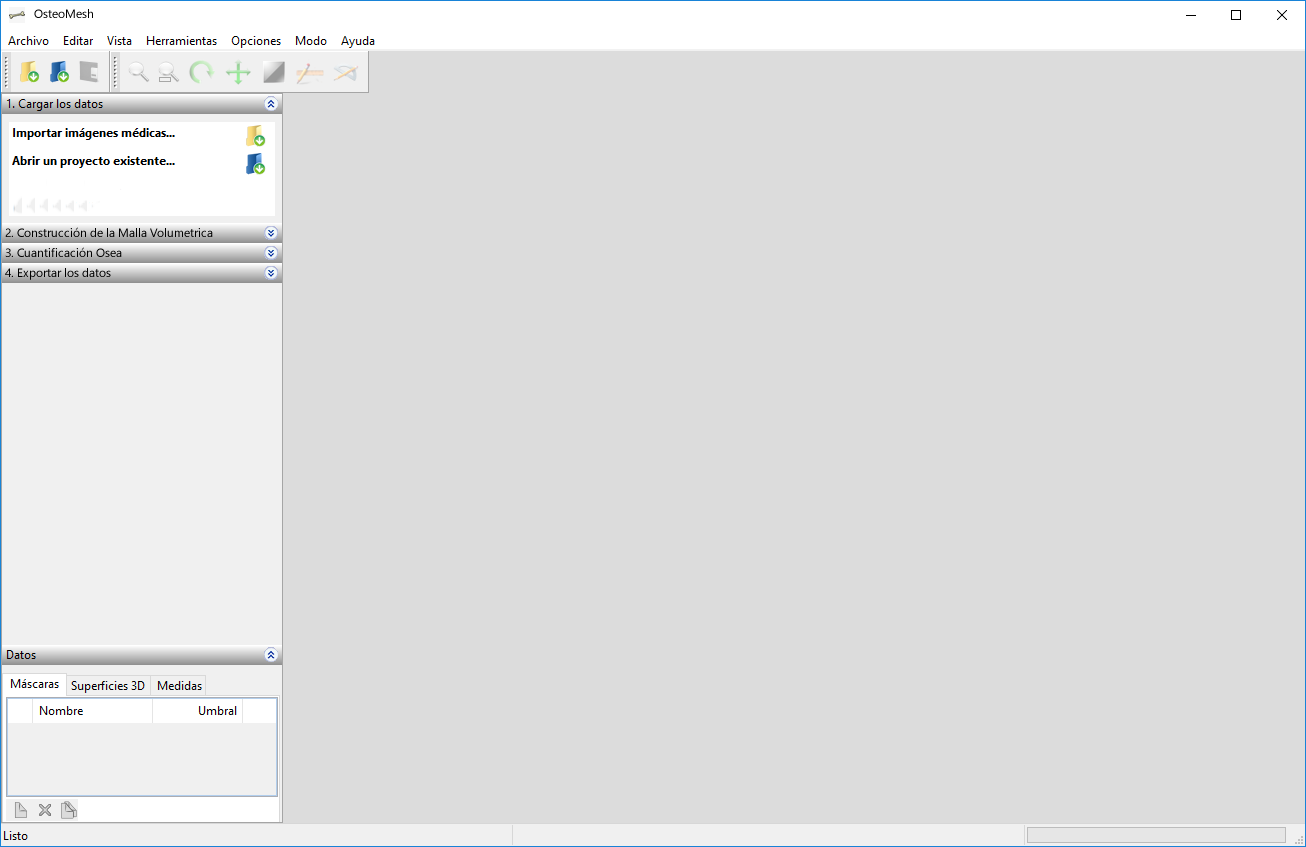
\includegraphics[width=\textwidth]{images/handling/1}
	\caption{Pantalla inicial}
	\label{fig:handling:1}
\end{figure}

\begin{figure}[!ht]
	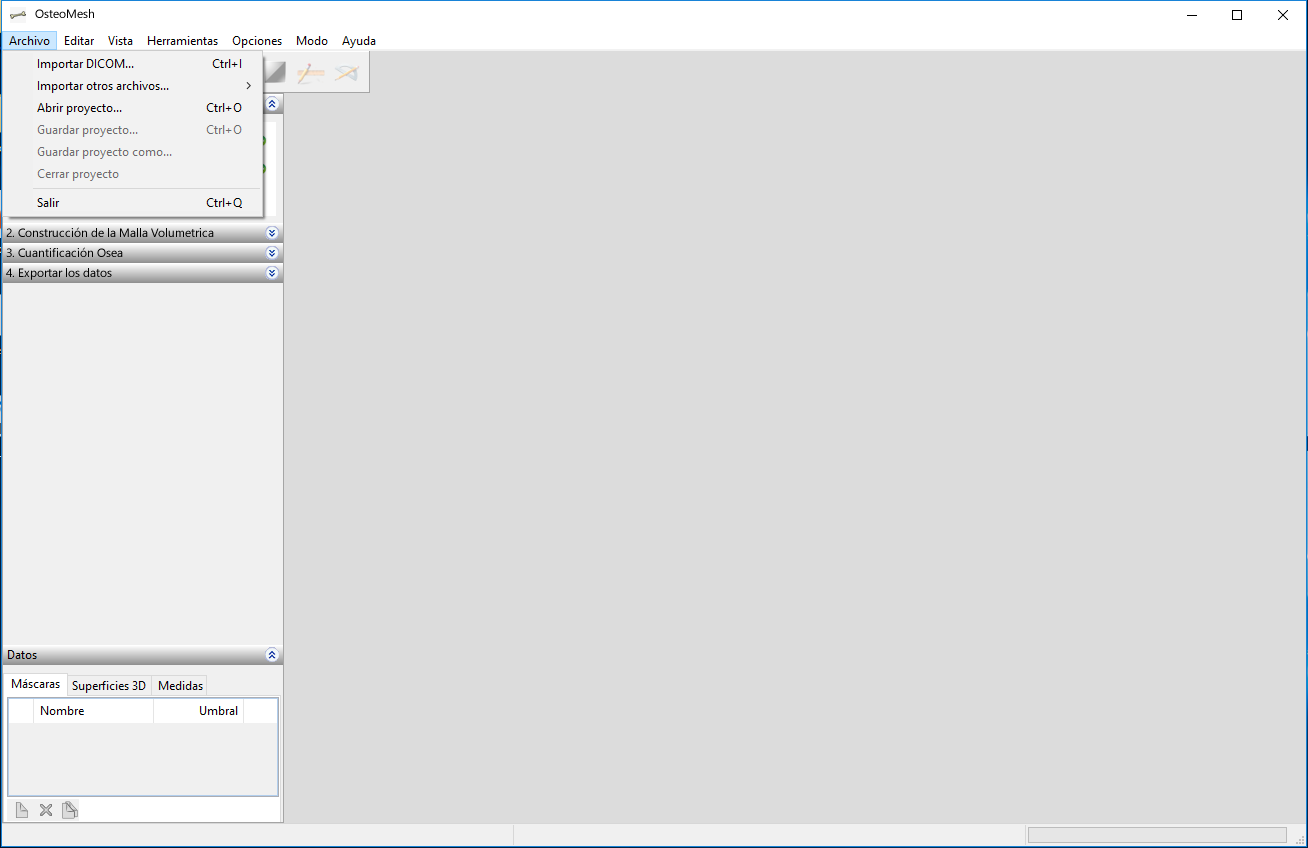
\includegraphics[width=\textwidth]{images/handling/2}
	\caption{Importar imagen volumétrica}
	\label{fig:handling:2}
\end{figure}

\begin{figure}[!ht]
	\centering
	\begin{subfigure}[b]{0.45\textwidth}
		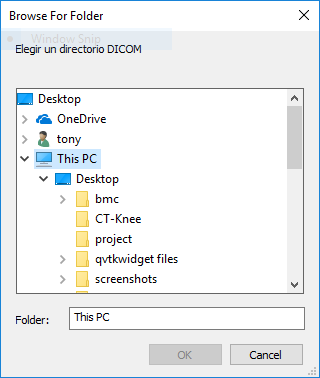
\includegraphics[width=\textwidth]{images/handling/3}
		\caption{Explorador de archivos} 
	\end{subfigure}
	\begin{subfigure}[b]{0.45\textwidth}
		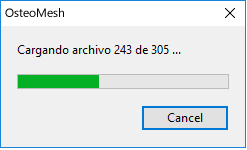
\includegraphics[width=\textwidth]{images/handling/4}
		\caption{Almacenamiento de archivo seleccionado} 
	\end{subfigure}
	\caption{A}
	\label{fig:brahand:segments}
\end{figure}

\begin{figure}[!ht]
	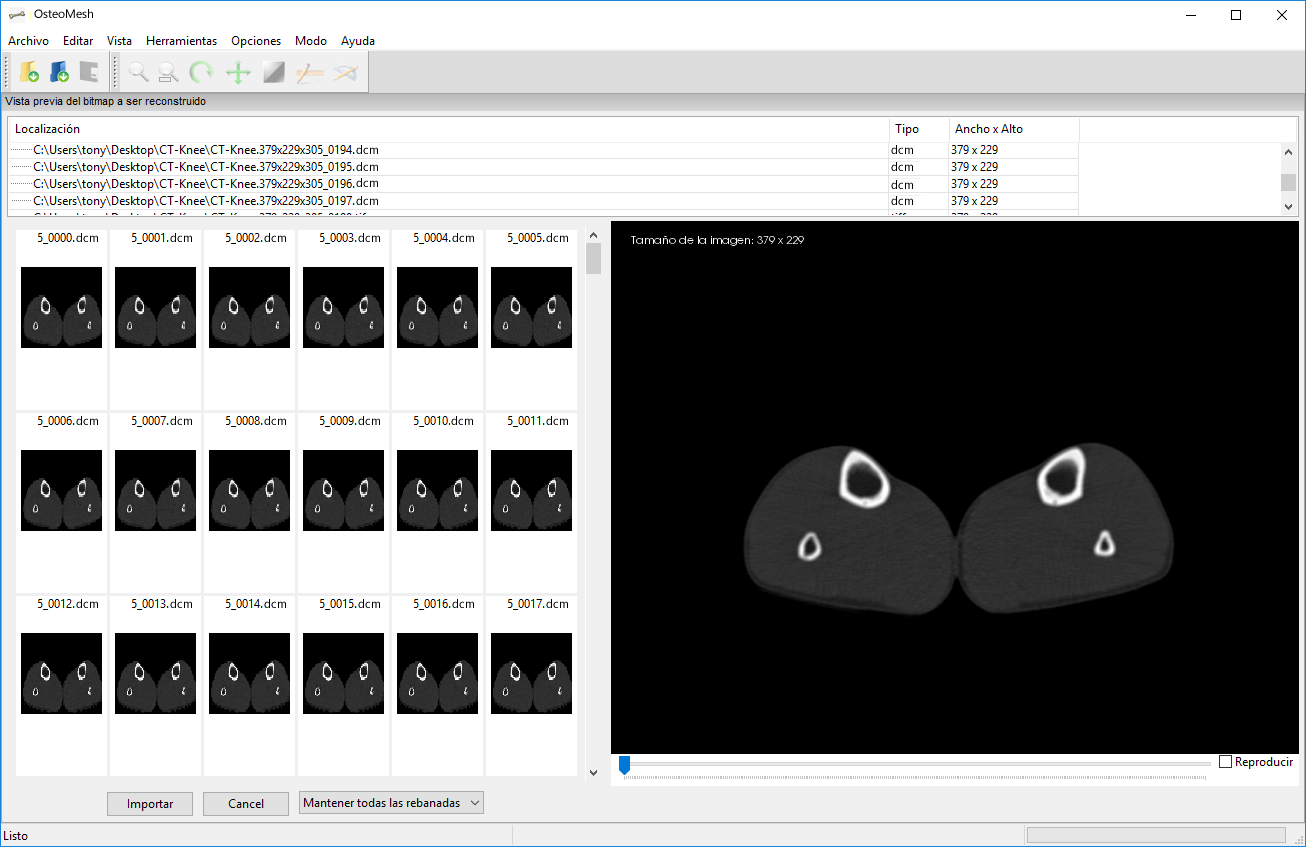
\includegraphics[width=\textwidth]{images/handling/5}
	\caption{Visualización de imagen volumétrica}
	\label{fig:handling:2}
\end{figure}

\newpage
\subsection{Construcción}
\label{interface:construction}
%Desarrollar una Interfaz con el algoritmo de creación de modelos de huesos

\subsection{Análisis}
\label{interface:analysis}
%Desarrollar una Interfaz de usuario final diseñada para el uso del Personal Médico y especialistas.

%\section{Desarrollar una Interfaz computacional con operaciones básicas de interacción con modelos tridimensionales}

\end{document}
